\documentclass[aspectratio=169]{beamer}

\usepackage[utf8]{inputenc}
\usepackage[T1]{fontenc}
\usepackage[spanish,es-tabla]{babel}
\decimalpoint

\usepackage{amsmath,amssymb}
\usepackage{booktabs}
\usepackage{graphicx}
\usepackage{tikz}
\usetikzlibrary{arrows.meta,positioning,babel}
\usepackage{hyperref}

% ============================================================================
% TEMA Y PALETA INSTITUCIONAL
% ============================================================================
\usetheme{Madrid}
\usecolortheme{default}

\definecolor{uniazul}{HTML}{0F294A}
\definecolor{uniacento}{HTML}{1D4ED8}
\definecolor{unialerta}{HTML}{DC2626}
\definecolor{univerde}{HTML}{15803D}
\definecolor{unifondo}{HTML}{F8FAFC}

\setbeamercolor{structure}{fg=uniazul}
\setbeamercolor{palette primary}{bg=uniazul,fg=white}
\setbeamercolor{palette secondary}{bg=uniacento,fg=white}
\setbeamercolor{palette tertiary}{bg=uniazul!85!black,fg=white}
\setbeamercolor{titlelike}{bg=uniazul,fg=white}
\setbeamercolor{block title}{bg=uniazul,fg=white}
\setbeamercolor{block body}{bg=unifondo,fg=black}
\setbeamercolor{block title alerted}{bg=unialerta,fg=white}
\setbeamercolor{block body alerted}{bg=red!5,fg=black}

\setbeamertemplate{navigation symbols}{}

\title[Alerta Temprana y Ruteo de Arroyos]{Sistema Colaborativo de Alerta Temprana y Ruteo Seguro Frente a Arroyos en el Corredor Uninorte--Mallorquín}
\subtitle{Matemáticas Discretas (NRC 3230) --- Grupo 1}
\author[Grupo 1]{%
    Jesús De León Jiménez \and Samuel De Oro Torres \and Karvin García Polo \\
    Juan Sierra Varela \and Andrés Torres García%
}
\institute[Uninorte]{%
    Universidad del Norte --- Departamento de Ciencias Básicas e Ingeniería \\
    Profesor: \textbf{Iván Yesid Gómez Gómez} \\
    \vspace{0.2cm}
    \small \textbf{Repositorio GitHub:} \url{https://github.com/Andrestcrack/Proyecto-arroyo}
}
\date{Noviembre de 2026}

\begin{document}

% ============================================================================
% DIAPOSITIVA 1: PORTADA
% ============================================================================
\begin{frame}[plain]
    \titlepage
\end{frame}

% ============================================================================
% DIAPOSITIVA 2: AGENDA Y DISTRIBUCIÓN EQUITATIVA (10 MINUTOS)
% ============================================================================
\begin{frame}{Agenda de Sustentación (10 Minutos --- 2 Minutos por Expositor)}
    \footnotesize
    \setlength{\tabcolsep}{4pt}
    \begin{tabular}{@{}cllc@{}}
        \toprule
        \textbf{Bloque} & \textbf{Expositor} & \textbf{Temática Principal} & \textbf{Tiempo} \\
        \midrule
        1 & \textbf{Jesús De León Jiménez} & Problema, impacto urbano, objetivos y alcance & 2:00 \\
        2 & \textbf{Samuel De Oro Torres} & Conjuntos, consenso $C(R,k)$, estados y Digrafo DAG & 2:00 \\
        3 & \textbf{Karvin García Polo} & Teoría de Grafos (Unidad 3): grados, $G-N_7$ y MST & 2:00 \\
        4 & \textbf{Juan Sierra Varela} & Redes (Unidad 4), BFS preventivo y desvío Dijkstra & 2:00 \\
        5 & \textbf{Andrés Torres García} & Software, mapa web (25 nodos), pruebas y conclusiones & 2:00 \\
        \bottomrule
    \end{tabular}

    \vspace{0.4cm}
    \begin{block}{Acceso al Código Fuente y Reproducibilidad}
        Todo el código ejecutable en Python puro, pruebas unitarias (\texttt{unittest}) y documentación técnica se encuentran alojados en: \\
        \centering \textbf{\url{https://github.com/Andrestcrack/Proyecto-arroyo}}
    \end{block}
\end{frame}

% ============================================================================
% BLOQUE 1: JESÚS DE LEÓN JIMÉNEZ (0:00 - 2:00)
% ============================================================================
\section{1. Problema y Objetivos (Jesús De León)}

\begin{frame}{1. Problema Real en Barranquilla y Entorno Uninorte}
    \framesubtitle{Expositor: Jesús De León Jiménez}
    \begin{columns}[T]
        \begin{column}{0.53\textwidth}
            \footnotesize
            \begin{alertblock}{¿Qué ocurre durante las lluvias?}
                La escorrentía pluvial convierte ejes críticos en \textbf{arroyos peligrosos}:
                \begin{itemize}
                    \item Av. Circunvalar y Cra 51B (Puerta 1 Uninorte).
                    \item Cra 53 (Rotonda Makro -- Portoazul).
                    \item Villa Campestre, canal colector, Arroyo León y Ciénaga de Mallorquín.
                \end{itemize}
            \end{alertblock}
            \begin{block}{Problemas Detectados}
                \begin{itemize}
                    \item \textbf{Riesgo vial:} vehículos atrapados sin alerta temprana.
                    \item \textbf{Falsas alarmas:} reportes aislados sin verificar.
                    \item \textbf{Falta de desvíos:} sin rutas dinámicas por calles transitables.
                \end{itemize}
            \end{block}
        \end{column}
        \begin{column}{0.44\textwidth}
            \centering
            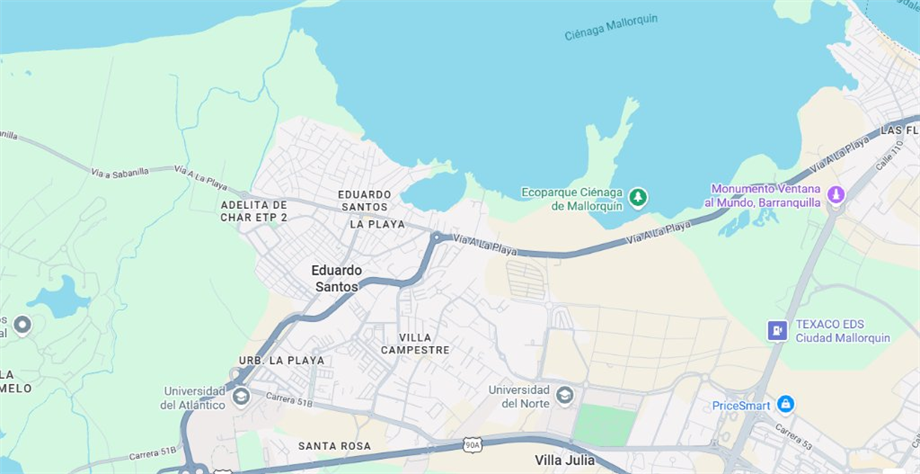
\includegraphics[width=0.96\textwidth]{mapa_barranquilla_google.png}
            \vspace{0.1cm}
            {\scriptsize Corredor geográfico Uninorte--Arroyo León--Mallorquín.}
        \end{column}
    \end{columns}
\end{frame}

\begin{frame}{1. Objetivos y Propuesta del Sistema}
    \framesubtitle{Expositor: Jesús De León Jiménez}
    \begin{block}{Objetivo General}
        Modelar e implementar un sistema colaborativo de alerta temprana y cálculo de rutas seguras fundamentado formalmente en \textbf{Matemáticas Discretas (NRC 3230)}.
    \end{block}

    \begin{columns}[T]
        \begin{column}{0.48\textwidth}
            \begin{block}{Pilares de Modelación}
                \begin{enumerate}
                    \item Conjuntos y lógica booleana para validar reportes ciudadanos sin duplicados.
                    \item Digrafo acíclico ponderado $G=(V,E)$ para el escurrimiento hidráulico.
                    \item Análisis de centralidad y vulnerabilidad estructural.
                \end{enumerate}
            \end{block}
        \end{column}
        \begin{column}{0.48\textwidth}
            \begin{block}{Solución Entregable}
                \begin{itemize}
                    \item \textbf{App de Escritorio:} simulación interactiva + auditoría formal completa.
                    \item \textbf{Mapa Web estilo Google Maps:} $25$ nodos arteriales y $31$ corredores con ruteo por calles reales.
                    \item \textbf{Sin librerías externas:} $100\%$ biblioteca estándar de Python.
                \end{itemize}
            \end{block}
        \end{column}
    \end{columns}
\end{frame}

% ============================================================================
% BLOQUE 2: SAMUEL DE ORO TORRES (2:00 - 4:00)
% ============================================================================
\section{2. Modelación Discreta (Samuel De Oro)}

\begin{frame}{2. Conjuntos, Consenso Booleano y Estados Discretos}
    \framesubtitle{Expositor: Samuel De Oro Torres}
    \begin{columns}[T]
        \begin{column}{0.47\textwidth}
            \begin{block}{Validación por Conjuntos}
                Para cada vértice $v \in V$, se almacena el conjunto de reportantes únicos $R_v \subseteq U$:
                \[
                    C(R_v, k) \equiv \bigl(|R_v| \ge k\bigr) \in \{\text{F}, \text{V}\}
                \]
                \begin{itemize}
                    \item Con $k = 3$: $1$ o $2$ reportes no bloquean la vía (\textbf{NARANJA}).
                    \item Con $|R_v| \ge 3$: consenso validado (\textbf{ROJO}).
                    \item Propiedad de conjunto: $R_v \cup \{c\} = R_v$ evita spam del mismo usuario.
                \end{itemize}
            \end{block}
        \end{column}
        \begin{column}{0.51\textwidth}
            \begin{block}{Función de Transición $f: Q \times \Sigma \to Q$}
                \tiny
                \setlength{\tabcolsep}{3pt}
                \begin{tabular}{@{}lllll@{}}
                    \toprule
                    \textbf{Estado $q$} & \textbf{REPORTE} & \textbf{ALERTA} & \textbf{CONSENSO} & \textbf{REINICIO} \\
                    \midrule
                    VERDE    & NARANJA & AMARILLO & ROJO & VERDE \\
                    AMARILLO & NARANJA & AMARILLO & ROJO & VERDE \\
                    NARANJA  & NARANJA & NARANJA  & ROJO & VERDE \\
                    ROJO     & ROJO    & ROJO     & ROJO & VERDE \\
                    \bottomrule
                \end{tabular}
            \end{block}
            \begin{itemize}
                \footnotesize
                \item $4$ estados discretos: \textcolor{univerde}{\textbf{VERDE}}, \textcolor{yellow!60!orange}{\textbf{AMARILLO}}, \textcolor{orange!90!black}{\textbf{NARANJA}} y \textcolor{unialerta}{\textbf{ROJO}}.
                \item \textbf{ROJO} absorbe nuevos reportes hasta \texttt{REINICIO}.
            \end{itemize}
        \end{column}
    \end{columns}
\end{frame}

\begin{frame}{2. Cuenca Hidráulica como Digrafo Acíclico (DAG)}
    \framesubtitle{Expositor: Samuel De Oro Torres}
    \begin{columns}[T]
        \begin{column}{0.62\textwidth}
            \centering
            \begin{tikzpicture}[
                >=Stealth, scale=0.82, transform shape,
                nodo/.style={circle, draw=uniazul, thick, fill=blue!6, minimum size=0.8cm, font=\footnotesize\bfseries},
                rojo/.style={circle, draw=unialerta, very thick, fill=red!12, minimum size=0.8cm, font=\footnotesize\bfseries},
                sumidero/.style={circle, draw=univerde, very thick, fill=green!10, minimum size=0.8cm, font=\footnotesize\bfseries},
                arista/.style={->, thick, draw=uniazul},
                corredor/.style={dashed, thick, draw=gray}
            ]
                \node[nodo] (N1) at (0,2.4) {$N_1$};
                \node[nodo] (N2) at (0,0) {$N_2$};
                \node[nodo] (N4) at (2.2,2.4) {$N_4$};
                \node[nodo] (N3) at (2.2,0) {$N_3$};
                \node[nodo] (N5) at (4.4,3.1) {$N_5$};
                \node[nodo] (N6) at (4.4,1.6) {$N_6$};
                \node[rojo] (N7) at (6.6,1.2) {$N_7$};
                \node[nodo] (N8) at (8.4,1.2) {$N_8$};
                \node[sumidero] (N9) at (10.2,1.2) {$N_9$};

                \draw[arista] (N1) -- node[above,font=\tiny]{450m} (N4);
                \draw[arista] (N2) -- node[below,font=\tiny]{380m} (N3);
                \draw[arista] (N4) -- node[above left,font=\tiny]{320m} (N5);
                \draw[arista] (N4) -- node[below left,font=\tiny]{620m} (N6);
                \draw[arista] (N5) -- node[above,font=\tiny]{740m} (N7);
                \draw[arista] (N6) -- node[below,font=\tiny]{510m} (N7);
                \draw[arista] (N3) -- node[below,font=\tiny]{1150m} (N7);
                \draw[arista] (N7) -- node[above,font=\tiny]{890m} (N8);
                \draw[arista] (N8) -- node[above,font=\tiny]{1450m} (N9);
                \draw[corredor] (N1) -- node[left,font=\tiny]{520m} (N2);
                \draw[corredor] (N3) -- node[right,font=\tiny]{480m} (N5);
            \end{tikzpicture}
            \vspace{0.15cm}
            {\scriptsize Línea continua: arcos dirigidos de escorrentía $|E|=9$. Línea discontinua: desvíos viales extra.}
        \end{column}
        \begin{column}{0.36\textwidth}
            \begin{block}{Orden Topológico (Kahn)}
                \footnotesize
                $\pi = (N_1, N_2, N_4, N_3, \allowbreak N_5, N_6, N_7, N_8, N_9)$
                \vspace{0.15cm}
                \begin{itemize}
                    \item Sin ciclos dirigidos: el agua siempre avanza aguas abajo.
                    \item Camino crítico ($L=5$): $N_1 \to N_4 \to N_5 \to N_7 \to N_8 \to N_9$.
                \end{itemize}
            \end{block}
        \end{column}
    \end{columns}
\end{frame}

% ============================================================================
% BLOQUE 3: KARVIN GARCÍA POLO (4:00 - 6:00)
% ============================================================================
\section{3. Teoría de Grafos --- Unidad 3 (Karvin García)}

\begin{frame}{3. Propiedades Formales de Grafos (Unidad 3)}
    \framesubtitle{Expositor: Karvin García Polo}
    \begin{columns}[T]
        \begin{column}{0.49\textwidth}
            \footnotesize
            \begin{block}{Lema del Apretón de Manos y Grados}
                \begin{itemize}
                    \item $|V| = 9$ vértices, $|E| = 9$ aristas.
                    \item No dirigido: $\delta(G)=1$, $\Delta(G)=4$ ($N_7$).
                    \item $\sum_{v \in V}\deg(v) = 18 = 2|E| = 2(9)$.
                    \item Dirigido: $\sum \deg^- = \sum \deg^+ = 9$.
                \end{itemize}
            \end{block}
            \begin{block}{Bipartición y Planaridad}
                \begin{itemize}
                    \item \textbf{Bipartito:} $V_1=\{N_1,N_3,N_5,N_6,N_8\}$, $V_2=\{N_2,N_4,N_7,N_9\}$ (ciclo par de long. $4$).
                    \item \textbf{Plano (Euler):} $V - E + F = 9 - 9 + 2 = 2$; $m = 9 \le 2n - 4 = 14$.
                \end{itemize}
            \end{block}
        \end{column}
        \begin{column}{0.48\textwidth}
            \footnotesize
            \begin{alertblock}{Subgrafo Inducido $G - N_7$ (Vulnerabilidad)}
                Al remover $N_7$ (\textit{Canal Colector}):
                \begin{itemize}
                    \item Quedan $8$ vértices y $5$ aristas.
                    \item Se fragmenta en \textbf{$3$ componentes}: $\{N_1,N_4,N_5,N_6\}$, $\{N_2,N_3\}$, $\{N_8,N_9\}$.
                    \item \textbf{Conclusión:} $N_7$ es \textbf{punto de articulación}; aísla $6$ sectores respecto a $N_9$.
                \end{itemize}
            \end{alertblock}
            \begin{block}{Árbol de Expansión Mínimo (MST)}
                Kruskal y Prim coinciden en \textbf{$8$ aristas} y costo óptimo de \textbf{$5\,770\text{ m}$} (descartando $(N_5, N_7)$ de $740\text{ m}$).
            \end{block}
        \end{column}
    \end{columns}
\end{frame}

% ============================================================================
% BLOQUE 4: JUAN SIERRA VARELA (6:00 - 8:00)
% ============================================================================
\section{4. Redes y Algoritmos (Juan Sierra)}

\begin{frame}{4. Análisis de Redes y Centralidades (Unidad 4)}
    \framesubtitle{Expositor: Juan Sierra Varela}
    \begin{columns}[T]
        \begin{column}{0.58\textwidth}
            \scriptsize
            \begin{tabular}{@{}ccccccc@{}}
                \toprule
                \textbf{Nodo} & $\deg(v)$ & $C_D(v)$ & $\sum d$ & $C_C(v)$ & $H_{\text{dir}}$ & $C_B^{\text{norm}}$ \\
                \midrule
                $N_1$ & 1 & 0.125 & 26 & 0.308 & 0.348 & 0.000 \\
                $N_2$ & 1 & 0.125 & 25 & 0.320 & 0.260 & 0.000 \\
                $N_3$ & 2 & 0.250 & 18 & 0.444 & 0.229 & 0.250 \\
                $N_4$ & 3 & 0.375 & 19 & 0.421 & \textbf{0.385} & 0.268 \\
                $N_5$ & 2 & 0.250 & 16 & 0.500 & 0.229 & 0.179 \\
                $N_6$ & 2 & 0.250 & 16 & 0.500 & 0.229 & 0.179 \\
                \textbf{$N_7$} & \textbf{4} & \textbf{0.500} & \textbf{13} & \textbf{0.615} & 0.188 & \textbf{0.732} \\
                $N_8$ & 2 & 0.250 & 18 & 0.444 & 0.125 & 0.250 \\
                $N_9$ & 1 & 0.125 & 25 & 0.320 & 0.000 & 0.000 \\
                \bottomrule
            \end{tabular}
        \end{column}
        \begin{column}{0.39\textwidth}
            \begin{block}{Interpretación de Red}
                \small
                \begin{itemize}
                    \item Diámetro geodésico: $D(G_u) = 5$.
                    \item \textbf{$N_7$ lidera las 3 centralidades:} grado ($0.500$), cercanía ($0.615$) e intermediación ($0.732$).
                    \item \textbf{$N_4$ lidera $H_{\text{dir}} = 0.385$:} mayor alcance preventivo aguas abajo.
                    \item Red bipartita \textit{Ciudadanos--Nodos} revela reportes simultáneos.
                \end{itemize}
            \end{block}
        \end{column}
    \end{columns}
\end{frame}

\begin{frame}{4. Algoritmos en Acción: Propagación BFS y Desvío por Dijkstra}
    \framesubtitle{Expositor: Juan Sierra Varela}
    \begin{columns}[T]
        \begin{column}{0.48\textwidth}
            \begin{block}{1. Alerta Preventiva por BFS ($\mathcal{O}(|V|+|E|)$)}
                Si $N_4$ (Puerta 1 Uninorte) alcanza consenso $k=3 \implies$ pasa a \textbf{ROJO} y propaga \textbf{AMARILLO} por capas:
                \begin{itemize}
                    \item \textbf{Capa 1:} $N_5$ (Campus), $N_6$ (Villa Campestre).
                    \item \textbf{Capa 2:} $N_7$ (Canal Colector).
                    \item \textbf{Capa 3:} $N_8$ (Arroyo León).
                    \item \textbf{Capa 4:} $N_9$ (Ciénaga de Mallorquín).
                \end{itemize}
            \end{block}
        \end{column}
        \begin{column}{0.49\textwidth}
            \begin{alertblock}{2. Ruteo Seguro en Subgrafo $G_{\text{vial}} - V_{\text{bloq}}$}
                Trayecto \textbf{Circunvalar ($N_1$) $\to$ Villa Campestre ($N_6$)}:
                \begin{itemize}
                    \item \textbf{Sin arroyos:} $N_1 \to N_4 \to N_6$ ($1\,070\text{ m}$, $4.3\text{ min}$).
                    \item \textbf{Con $N_4$ inundado:} Dijkstra elimina $N_4$ y recalcula por Cra 53:
                    \[
                        N_1 \to N_2 \to N_3 \to N_7 \to N_6
                    \]
                    ($2\,560\text{ m}$, $10.2\text{ min}$ --- desvío seguro garantizado).
                \end{itemize}
            \end{alertblock}
        \end{column}
    \end{columns}
\end{frame}

% ============================================================================
% BLOQUE 5: ANDRÉS TORRES GARCÍA (8:00 - 10:00)
% ============================================================================
\section{5. Implementación, Demo y Conclusiones (Andrés Torres)}

\begin{frame}{5. Arquitectura Ejecutable y Escalamiento Web (25 Nodos)}
    \framesubtitle{Expositor: Andrés Torres García}
    \begin{columns}[T]
        \begin{column}{0.53\textwidth}
            \begin{block}{Dos Entornos Conectados en Python Puro}
                \begin{itemize}
                    \item \textbf{App de Escritorio (\texttt{interfaz\_app.py}):} mapa interactivo Uninorte, controles de consenso $k$, animación BFS, ruteo Dijkstra y auditoría Unidad 3 y 4.
                    \item \textbf{Servidor Web (\texttt{servidor\_web\_arroyos.py}):} vista tipo Google Maps con \textbf{$25$ nodos} ($9$ cuenca + $16$ arterias de Barranquilla: Vía 40, Cra 51B, Cra 53, Cra 46, Cll 84/76/72, Murillo, Cll 30, Circunvalar), \textbf{$31$ corredores} y \textbf{$71$ polilíneas OSM} precargadas calle por calle.
                \end{itemize}
            \end{block}
        \end{column}
        \begin{column}{0.44\textwidth}
            \centering
            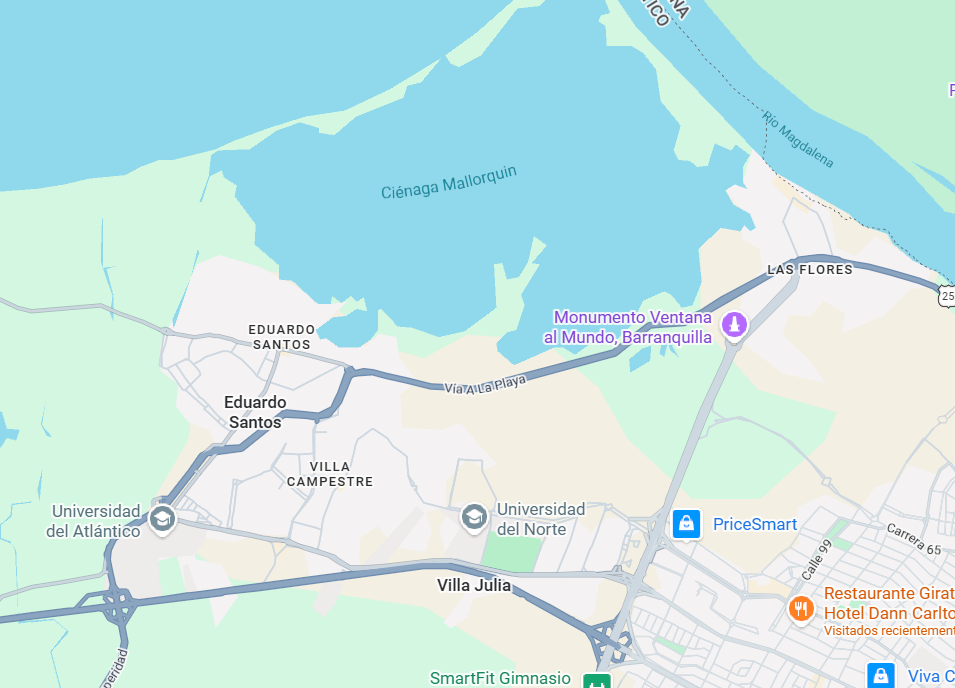
\includegraphics[width=\textwidth]{mapa_panoramico_uninorte.png}
            \vspace{0.1cm}
            {\scriptsize Vista panorámica Vía a la Playa -- Uninorte -- Eduardo Santos.}
        \end{column}
    \end{columns}
\end{frame}

\begin{frame}{5. Pruebas Unitarias, Conclusiones y Limitaciones}
    \framesubtitle{Expositor: Andrés Torres García}
    \begin{columns}[T]
        \begin{column}{0.48\textwidth}
            \footnotesize
            \begin{block}{Verificación Automatizada}
                \texttt{python -m unittest test\_arroyos.py -v}:
                \begin{itemize}
                    \item \textbf{$14/14$ pruebas aprobadas (\texttt{OK})} en $0.012\text{ s}$.
                    \item Verifican consenso, estados, TAM, bipartición, $G - N_7$, Kruskal/Prim, centralidades y Dijkstra.
                \end{itemize}
            \end{block}
            \begin{block}{Conclusión Principal}
                Grafos y Redes transforman reportes dispersos en prevención hidráulica y rutas seguras reproducibles.
            \end{block}
        \end{column}
        \begin{column}{0.49\textwidth}
            \footnotesize
            \begin{alertblock}{Limitaciones y Trabajo Futuro}
                \begin{itemize}
                    \item Sin sensores IoT físicos ni pluviómetros conectados aún.
                    \item Cobertura concentrada en vías arteriales principales ($25$ nodos).
                    \item Trazado dinámico fuera de los $71$ corredores cacheados depende de OSRM en línea.
                \end{itemize}
            \end{alertblock}
            \vspace{0.1cm}
            \centering
            \textbf{Repositorio GitHub (código y README):} \\
            \scriptsize\url{https://github.com/Andrestcrack/Proyecto-arroyo}
        \end{column}
    \end{columns}
\end{frame}

% ============================================================================
% DIAPOSITIVA FINAL: DEMO Y PREGUNTAS
% ============================================================================
\begin{frame}[plain]
    \centering
    \vspace{1.2cm}
    {\Huge \color{uniazul} \textbf{¡Muchas Gracias!}} \\[0.5cm]
    {\Large Sesión de Preguntas y Demostración en Vivo} \\[0.8cm]
    \begin{block}{Ejecución Rápida y Código Fuente}
        \centering
        \texttt{python arroyos\_uninorte.py} \quad | \quad \texttt{python -m unittest test\_arroyos.py -v} \\[0.2cm]
        \textbf{\url{https://github.com/Andrestcrack/Proyecto-arroyo}}
    \end{block}
    \vspace{0.3cm}
    {\small Matemáticas Discretas (NRC 3230) --- Prof. Iván Yesid Gómez Gómez --- Grupo 1}
\end{frame}

\end{document}
